\documentclass{article}
\usepackage[utf8]{inputenc}
\usepackage{amsmath}
\usepackage{amssymb}
\usepackage{amsthm}
\usepackage{enumerate}
\usepackage{mathtools}
\usepackage{float} % For plassering av bilder
\usepackage{a4wide} % mer width
\usepackage{amsmath}
\usepackage{amssymb}
\usepackage{parskip}

\usepackage[colorlinks=false,allcolors=blue]{hyperref}
%Fikser hyperref
\addto\extrasnorsk{%
\def\figureautorefname{Figure}%
\def\tableautorefname{Table}%
\def\sectionautorefname{section}%
\def\subsectionautorefname{subsection}%
}
% Vi endrer fonten som brukes for URLer til den vanlige tekstfonten.
\urlstyle{same}


% FRA IC
\usepackage{natbib}
\usepackage{amsmath}
\usepackage{listings}
\usepackage{graphicx}
\usepackage[inline]{enumitem}
\usepackage{xcolor}
 \usepackage{booktabs}
\date{}
\newcommand*{\boxednumber}[1]{%
    \expandafter\readdigit\the\numexpr#1\relax\relax
}
\newcommand*{\readdigit}[1]{%
    \ifx\relax#1\else
        \boxeddigit{#1}%
        \expandafter\readdigit
    \fi
}
% Format macro used for every digit, adjust to your liking:
\newcommand*{\boxeddigit}[1]{\fbox{#1}\hspace{-\fboxrule}}

\usepackage[left=4cm,right=4cm,vmargin=1.5cm,footnotesep=0.5cm]{geometry}
\setlength\parindent{0pt}



\title{TDT4265 - Computer Vision and Deep Learning \\Assignment 2}
\author{Jakob Vahlin & Kristian Stensgård}
%\date{September 2020}

\begin{document}

\maketitle

\tableofcontents
\newpage

\section{Softmax regression with backpropagation}
\subsection{Task 1a: Backpropagation}

\subsubsection*{i)}

In the neural network considered in this assignment the gradient descent update rule for weights $w_{ji}$ of the \textbf{hidden} layer is given by

\begin{equation}
    w_{j i}:=w_{j i}-\alpha \frac{\partial C}{\partial w_{j i}} , \quad \alpha \in \mathbb{R}
    \label{eq:1a_start}
\end{equation}
where $C(w)$ is the cross entropy loss, defined by
\begin{equation}
    C(w)=\frac{1}{N} \sum_{n=1}^{N} C^{n}(w), \quad C^{n}(w)=-\sum_{k=1}^{K} y_{k}^{n} \ln \left(\hat{y}_{k}^{n}\right)
    \label{eq:cross_entropy}
\end{equation}
where $\hat{y}$ is the Softmax activation function for the \textit{output} layer, defined by

\begin{equation}
    \hat{y}_{k}=\frac{e^{z_{k}}}{\sum_{k^{\prime}}^{K} e^{z_{k^{\prime}}}}, \quad \text { where } z_{k}=w_{k}^{T} \cdot a=\sum_{j}^{J} w_{kj} \cdot a_{j}
    \label{eq:softmax}
\end{equation}

where $w_{kj}$ are weights in the output layer and $a_j = f(z_j)$ is the is the Sigmoid activation function  in the \textit{hidden} layer, defined as

\begin{equation}
    a_j =  f(z_j)=\frac{1}{1+e^{-z_j}}, \quad z_j = w_j^{T} x=\sum_{i}^{I} w_{ji} \cdot x_{i}
    \label{eq:sigmoid}
\end{equation}



By algebraic manipulation it can be shown that \eqref{eq:1a_start} can be written as

\begin{equation}
    w_{j i}:=w_{j i}-\alpha \delta_{j} x_{i}
    \label{eq:1a_goal}
\end{equation}

by defining $\delta_{j}=\frac{\partial C}{\partial z_{j}}$.

To derive the equvialent expression for the gradient descent update rule given by \eqref{eq:1a_goal} consider the partial derivative of the cross entropy loss function w.r.t the variable $w_{ji}$. From \eqref{eq:cross_entropy} and \eqref{eq:softmax} it is clear that $C(w)$ has a dependence on $z_k$. Furthermore, from \eqref{eq:softmax}, it is clear that $z_k$ in turn has a dependence on $a_j$, which in turn has a dependence on $z_j$, as evident from \eqref{eq:sigmoid}. Finally, from \eqref{eq:sigmoid} it is clear that $z_j$ has a dependence on $w_{ji}$. Consequently, the cost functions dependence on the variable $w_{ji}$ is ``chained together'' through the variables $z_k$,$a_j$ and $z_j$. By defining $\boldsymbol{z_{k}} = [z_1,z_2,\dots,z_K]$ as the vector containing $z$ values from the output layer, $\boldsymbol{a} = [a_1,a_2,\dots,a_J]$ as the vector with $a$ values from the hidden layer and $\boldsymbol{z_j} = [z_1,z_2,\dots,z_J]$ as the vector containing $z$ values from the hidden layer, we can express the cross entropy loss function in terms of its variables in the following way
\begin{align}
\begin{split}
    C(w) &= C(\boldsymbol{z_k}) \\ 
    &= C\big(\boldsymbol{z_k}(\boldsymbol{a})\big) \\
    &= C\bigg(\boldsymbol{z_k}\big(\boldsymbol{a}(\boldsymbol{z_j})\big)\bigg) \\
    &= C\bigg(\boldsymbol{z_k}\big(\boldsymbol{a}(\boldsymbol{z_j}(w))\big)\bigg)
    \label{eq:cost_var_def}
\end{split}
\end{align}

with $K$ representing the number of nodes in the output layer, and $J$ representing the number of nodes in the hidden layer. In this case, the lowercase $w$ represents the weight matrix from the input layer to the hidden layer, in accordance with the notation in the assignment description. Therefore, the derivative of the cross entropy loss function, w.r.t to any weight in the \textit{hidden} layer $w_{ji}$, $\frac{\partial C}{\partial w_{ji}}$, can be expressed by applying the multivariate chain rule.

In the following, to distinguish between $z$ vector from the different layers in the network, entries from the $z$ vector from the hidden layer will be labeled $z^j$ and entries from the $z$ vector from the output layer will be labeled $z^k$. This is needed to distinguish between i.e $z_{1}$ from the hidden layer and $z_1$ from the output layer.

\begin{align}
\begin{split}
    \frac{\partial C}{\partial w_{ji}} &= \frac{\partial C}{\partial z_1^k} \Bigg( 
    \frac{\partial z_1^k}{\partial a_1}\frac{\partial a_1}{\partial  z^j_1} \frac{\partial z^j_1}{\partial w_{1i}} + \frac{\partial z_1^k}{\partial a_2}\frac{\partial a_2}{\partial  z^j_2} \frac{\partial z^j_2}{\partial w_{2i}} + \dots + \frac{\partial z_1^k}{\partial a_J}\frac{\partial a_J}{\partial  z^j_J} \frac{\partial z^j_J}{\partial w_{Ji}}\Bigg) \\
    &+ \frac{\partial C}{\partial z_2^k} \Bigg( 
    \frac{\partial z_2^k}{\partial a_1}\frac{\partial a_1}{\partial  z^j_1} \frac{\partial z^j_1}{\partial w_{1i}} + \frac{\partial z_2^k}{\partial a_2}\frac{\partial a_2}{\partial  z^j_2} \frac{\partial z^j_2}{\partial w_{2i}} + \dots + \frac{\partial z_2^k}{\partial a_J}\frac{\partial a_J}{\partial  z^j_J} \frac{\partial z^j_J}{\partial w_{Ji}}\Bigg) \\
    &+ \dots + \frac{\partial C}{\partial z_K^k} \Bigg( 
    \frac{\partial z_K^k}{\partial a_1}\frac{\partial a_1}{\partial  z^j_1} \frac{\partial z^j_1}{\partial w_{1i}} + \frac{\partial z_1^k}{\partial a_2}\frac{\partial a_2}{\partial  z^j_2} \frac{\partial z^j_2}{\partial w_{2i}} + \dots + \frac{\partial z_1^k}{\partial a_J}\frac{\partial a_J}{\partial  z^j_J} \frac{\partial z^j_J}{\partial w_{Ji}}\Bigg) 
\end{split} \label{eq:chain}
\end{align}

Equation \eqref{eq:chain} can be simplified to a set of sums (\textit{Notation}: Note that as there no longer exist a need to distinguish between $z$ vectors from the different layers in the network, as this will now be clear from the variable ($j$ or $k$) used to index the vectors in accordance with the notation in the assignment description).   

\begin{equation}
    \frac{\partial C}{\partial w_{ji}} = \sum_{k=1}^K \frac{\partial C}{\partial z_k}\Bigg( \sum_{j'=1}^J \frac{\partial z_k}{\partial a_{j'}}\frac{\partial a_{j'}}{\partial z_{j'}}\frac{\partial z_{j'}}{\partial w_{ji}} \Bigg)
    \label{eq:chain_sum}
\end{equation}

To further simplify \eqref{eq:chain_sum}, consider the last partial derviative, $\frac{\partial z_{j'}}{\pratial w_{ji}}$. From the definition of $z_j$ given in \eqref{eq:sigmoid} the derivative w.r.t to $w_{ji}$ can be expressed as

\begin{equation}
    \frac{\partial z_{j'}}{\partial w_{ji}} = \frac{\partial}{\partial w_{ji}} \sum_{i'=1}^I w_{j'i'}x_{i'}, \quad \text{for a given \textit{j'}}
    \label{eq:diffzj}
\end{equation}

Similar to when deriving the gradients of the cost function in Assignment 1, the resulting differentiation of the sums in \eqref{eq:diffzj} w.r.t to a given given weight, $w_{j'i'}$ will only be non-zero for $j' = j$ and $i' = i$. When this is the case the differentiation of $z_{j'} = z_j$ becomes

\begin{align}
\begin{split}
    \frac{\partial z_{j}}{\partial w_{ji}} &= \frac{\partial }{\partial w_{ji}} \sum_{i'=1}^I w_{ji'}x_{i'} \\
    &= \frac{\partial}{\partial w_{ji}} w_{ji}x_i \\
    &= x_i
\end{split}
\label{eq:diffzjdone}
\end{align}
 
 Thus it is clear that $\frac{\partial z_{j'}}{\partial w_{ji}} = x_i$, for $j' = j$ and thus it is independent of the $j'$ and $k$ indecies. Consequently it can be moved outside of the sums that goes over all $j'$ and over all $k$.
 
\begin{align}
\begin{split}
    \frac{\partial C}{\partial w_{ji}} &= \sum_{k=1}^K \frac{\partial C}{\partial z_k}\Bigg( \sum_{j'=1}^J \frac{\partial z_k}{\partial a_{j'}}\frac{\partial a_{j'}}{\partial z_{j'}}\frac{\partial z_{j'}}{\partial w_{ji}} \Bigg) \\
    &=  \sum_{k=1}^K \frac{\partial C}{\partial z_k}\Bigg( \sum_{j'=1}^J \frac{\partial z_k}{\partial a_{j'}}\frac{\partial a_{j'}}{\partial z_{j'}}x_i \Bigg) \\
    &=  \Bigg(\sum_{k=1}^K \frac{\partial C}{\partial z_k}\Bigg( \sum_{j'=1}^J \frac{\partial z_k}{\partial a_{j'}}\frac{\partial a_{j'}}{\partial z_{j'}}\Bigg)\Bigg) x_i
    \label{eq:movexiout}
\end{split}
\end{align}

Furthermore, consider the definition of $\delta_j$, given by

\begin{equation}
    \delta_j = \frac{\partial C}{\partial z_j}
    \label{eq:deltadef}
\end{equation}
 
 From the chain of dependencies given in \eqref{eq:cost_var_def}, the derivative in \eqref{eq:deltadef} can be expressed by applying the multivariate chain rule
 
\begin{equation}
    \delta_j = \frac{\partial C}{\partial z_j} = \sum_{k=1}^K \frac{\partial C}{\partial z_k} \bigg(\sum_{j=1}^J\frac{\partial z_k}{\partial a_j}\frac{\partial a_j}{\partial z_j} \bigg)
    \label{eq:djchain}
\end{equation}
By inserting the result in \eqref{eq:djchain} into \eqref{eq:movexiout}, the derivative of the cost function w.r.t $w_{ji}$ becomes

\begin{align}
\begin{split}
     \frac{\partial C}{\partial w_{ji}} &= \Bigg(\sum_{k=1}^K \frac{\partial C}{\partial z_k}\Bigg( \sum_{j=1}^J \frac{\partial z_k}{\partial a_j}\frac{\partial a_j}{\partial z_j}\Bigg)\Bigg) x_i \\
     &= \frac{\partial C}{\partial z_j} x_i \\
     &= \delta_j x_i
\end{split}
\label{eq:dif_done}
\end{align}

Finally, inserting the result in \eqref{eq:dif_done} into \eqref{eq:1a_start}, the desired result given by \eqref{eq:1a_goal} is found. \qed

\subsubsection*{ii)}

With $\delta_j$ defined as

\begin{equation}
\delta_j = \frac{\partial C}{\partial z_j}
    \label{eq:deltaj}
\end{equation}
where $z_j$ is defined as in \eqref{eq:softmax}, it can be shown that $\delta_j$ can be expressed as

\begin{equation}
    \delta_j = f'(z_j)  \sum_{k=1}^K w_{kj} \delta_k
    \label{eq:part2goal}
\end{equation}
where $\delta_k = \frac{\partial C}{\partial z_k} = -(y_k - \hat{y}_k)$ and $f'(z_j) = \frac{\partial f}{\partial z_j} = \frac{\partial a_j}{\partial z_j}$ is the slope of the Sigmoid activation function for the hidden layer, given by \eqref{eq:softmax}.

To prove the relationship given by \eqref{eq:part2goal}, recall from part \textit{i)} and \eqref{eq:djchain} the definition of $\delta_j$ with the derivative written out according to the chain rule

\begin{equation}
        \delta_j = \frac{\partial C}{\partial z_j} = \sum_{k=1}^K \frac{\partial C}{\partial z_k} \bigg(\sum_{j'=1}^J\frac{\partial z_k}{\partial a_{j'}}\frac{\partial a_{j'}}{\partial z_j} \bigg)
    \label{eq:djchainagain}
\end{equation}

First, consider the term $\frac{\partial z_k}{a_{j'}}$ which, from the definition of $z_k$, can be expressed as
\begin{align}
\begin{split}
    \frac{\partial z_k}{\partial a_{j'}} &= \frac{\partial}{\partial a_{j'}} \sum_{j'' = 1}^J w_{kj''} \cdot a_{j''}, \quad \text{for a given \textit{k}}
\end{split}
\label{eq:zk_diff_aj}
\end{align}

Again, the expression in \eqref{eq:zk_diff_aj} is only non-zero for $j'' = j'$, in which the resulting expression becomes

\begin{align}
\begin{split}
    \frac{\partial z_k}{\partial a_{j'}} &= \frac{\partial}{\partial a_{j'}} \sum_{j'' = 1}^J w_{kj''} \cdot a_{j''} \\
    &=  \frac{\partial}{\partial a_{j'}} w_{kj'} \cdot a_{j'} \\
    &= w_{kj'}
\end{split}
\label{eq:diff_zk_done}
\end{align}

Inserting the result in \eqref{eq:diff_zk_done} into \eqref{eq:djchainagain} gives
\begin{align}
\begin{split}
        \delta_j &= \frac{\partial C}{\partial z_j} = \sum_{k=1}^K \frac{\partial C}{\partial z_k} \bigg(\sum_{j'=1}^J\frac{\partial z_k}{\partial a_{j'}}\frac{\partial a_{j'}}{\partial z_j} \bigg) \\
        &= \sum_{k=1}^K \frac{\partial C}{\partial z_k} \bigg(\sum_{j'=1}^J w_{kj'} \frac{\partial a_{j'}}{\partial z_j} \bigg)
\end{split}
\label{eq:dj_shorter}
\end{align}

Next, consider the expression $\sum_{j'=1}^J w_{kj'} \frac{\partial a_{j'}}{\partial z_j}$. Differentiating $a_{j'}$ w.r.t the variable $z_j$ will only be non-zero when $j' = j$. When this is the case, the resulting derivative becomes
\begin{align}
\begin{split}
    \sum_{j'=1}^J w_{kj'} \frac{\partial a_{j'}}{\partial z_j} &= w_{kj}\frac{\partial a_j}{\partial z_j} \\ &= w_{kj} f'(z_j)
\end{split}
\label{eq:diff_aj_zj}
\end{align}
since $a_j = f(z_j)$. Inserting the result in \eqref{eq:diff_aj_zj} into \eqref{eq:dj_shorter} gives

\begin{align}
\begin{split}
     \delta_j &= \sum_{k=1}^K \frac{\partial C}{\partial z_k} \bigg(\sum_{j'=1}^J w_{kj'} \frac{\partial a_{j'}}{\partial z_j} \bigg) \\
     &=\sum_{k=1}^K \frac{\partial C}{\partial z_k} \bigg( w_{kj} f'(z_j)\bigg)
\end{split}
\label{eq:almost_there}
\end{align}
Observe that $f'(z_j)$ is independent of $k$ and consequently can be moved outside the sum over all $k$. Finally, by the definition $\delta_k = \frac{\partial C}{\partial z_k}$ the desired expression for $\delta_j$ is achieved

\begin{equation}
    \delta_j = f'(z_j) \sum_{k=1}^K \delta_k w_{kj}
\end{equation}
\qed
\subsection{Task 1b: Vectorize computation}
\textit{Notation:} To represent matrices, a bold uppercase letter, i.e \textbf{W}, will be used. To represent vectors, a bold and italic lowercase letter, i.e $\boldsymbol{w}$, will be used. To represent a scalar, an italic lowercase letter, i.e $w$, will be used. 

Furthermore, the number of nodes in the input layer, will be labeled $I$. The number of nodes in the hidden layer will be labeled $J$. The number of nodes in the output layer will be labeled $K$.





\subsubsection*{i) The input layer to hidden layer} 
Using matrix notation, the update rule for the weight matrix from the input layer to hidden layer, $\text{\textbf{W}}_\textbf{1}$, becomes 
\begin{equation}
    \text{\textbf{W}}_\textbf{1} := \text{\textbf{W}}_\textbf{1} - \alpha \boldsymbol{\delta_J} \boldsymbol{x}^T, \quad \alpha \in \mathbb{R}
    \label{eq:matrix_hidden}
\end{equation}

The contents and dimensions of the matrices and vectors in \eqref{eq:matrix_hidden} are as follows: 

For the $\text{\textbf{W}}_\textbf{1}$ matrix:
\begin{equation}
    \text{\textbf{W}}_\textbf{1} =
    \begin{bmatrix}
        w_{11} & w_{12}& \dots & w_{1I} \\
         w_{21} & w_{22}& \dots & w_{2I} \\
        \vdots & \vdots & \ddots & \vdots \\
         w_{J1} & w_{J2}& \dots & w_{JI} \\
    \end{bmatrix}
    , \quad \text{\textbf{W}}_\textbf{1} \in \mathcal{M}_{J \times I}(\mathbb{R})
\end{equation}
where the matrix entries $w_{ji}$ are updated according to \eqref{eq:1a_goal}. In a network with an input layer of $I = 785$ units and one hidden layer with $J = 64$ units, the dimension of $\mathbf{W_1}$ becomes $[64 \times 785]$.

For the $\boldsymbol{\delta_J}$ vector:

\begin{equation}
    \boldsymbol{\delta_J} = 
    \begin{bmatrix}
        \delta_1 \\
        \delta_2 \\
        \vdots \\
        \delta_J
    \end{bmatrix}
    = \begin{bmatrix}
        f^{\prime}\left(z_{1}\right) \sum_{k=1}^K w_{k 1} \delta_{k} \\
        f^{\prime}\left(z_{2}\right) \sum_{k=1}^K w_{k 2} \delta_{k} \\
        \vdots \\
        f^{\prime}\left(z_{J}\right) \sum_{k=1}^K w_{k J} \delta_{k}
    \end{bmatrix}
    , \quad \boldsymbol{\delta_J} \in \mathbb{R}^J
    \label{eq:deltaJ_full}
\end{equation}

where $f'(z_j)$ is the derivative of the activation function and $\delta_k$ is the error vector found in \ref{eq:errorvec_k}. Using matrix notation the expression in \eqref{eq:deltaJ_full} becomes:

\begin{equation}
    \boldsymbol{\delta_J} = f'(\boldsymbol{z_J}) \odot \mathbf{W_2}^T \boldsymbol{\delta_K}, \quad \boldsymbol{\delta_J} \in \mathbb{R}^J
\end{equation}
In a network with $J = 64$ hidden units, the dimension of the $\boldsymbol{\delta_J}$ vector is [64\times1]

For the $\boldsymbol{x}$ vector:

\begin{equation}
    \boldsymbol{x} = 
    \begin{bmatrix}
        x_1 \\
        x_2 \\
        \vdots \\
        x_I
    \end{bmatrix}
    , \quad \boldsymbol{x} \in \mathbb{R}^I
\end{equation}
where the $x_i$ values are the pixel values in the image and one bias. In a network with $I = 784 + 1 = 785$ input unist, the dimension of the $\boldsymbol{x}$ vector is $[785\times1]$

Note that $\text{\textbf{A}} = \boldsymbol{\delta_J} \cdot \boldsymbol{x}^T$ will yield a matrix $\text{\textbf{A}} \in \mathcal{M}_{J \times I}(\mathbb{R})$ due to the fact that $\boldsymbol{x}$ vector is transposed in the vector product. Thus the matrix subtraction $\text{\textbf{W}}_\textbf{1} - \text{\textbf{A}}$ is valid, as both matrices are have dimension [$J \times I$].  

\subsubsection*{ii) The hidden layer to output layer} 
Using matrix notation, the update rule for the weight matrix from the hidden layer to output layer, $\text{\textbf{W}}_\textbf{2}$, becomes 
\begin{equation}
    \text{\textbf{W}}_\textbf{2} := \text{\textbf{W}}_\textbf{2} - \alpha \boldsymbol{\delta_K} \boldsymbol{a}^T,\quad \alpha \in \mathbb{R}
    \label{eq:matrix_output}
\end{equation}

The contents and dimensions of the matrices and vectors in \eqref{eq:matrix_output} are as follows: 


For the $\text{\textbf{W}}_\textbf{2}$ matrix:
\begin{equation}
    \text{\textbf{W}}_\textbf{2} =
    \begin{bmatrix}
        w_{11} & w_{12}& \dots & w_{1I} \\
         w_{21} & w_{22}& \dots & w_{2I} \\
        \vdots & \vdots & \ddots & \vdots \\
         w_{J1} & w_{J2}& \dots & w_{JI} \\
    \end{bmatrix}
    , \quad \text{\textbf{W}}_\textbf{2} \in \mathcal{M}_{K \times J}(\mathbb{R})
\end{equation}
where the matrix entries $w_{ji}$ are updated according to $w_{k j}:=w_{k j}-\alpha \delta_{k} a_{j}$.

In a network layer with $J = 64$ hidden units and $K = 10$ output units, the dimension of $\mathbf{W_2}$ becomes $[10\times64]$.

For the $\boldsymbol{\delta_K}$ vector:

\begin{equation}
    \boldsymbol{\delta_K} = 
    \begin{bmatrix}
        \delta_1 \\
        \delta_2 \\
        \vdots \\
        \delta_K
    \end{bmatrix}
    = \begin{bmatrix}
        -(y_1 - \hat{y}_1) \\
        -(y_2 - \hat{y}_2)\\
        \vdots \\
        -(y_K - \hat{y}_K)
    \end{bmatrix}
    , \quad \boldsymbol{\delta_K} \in \mathbb{R}^K
    \label{eq:errorvec_k}
\end{equation}

where $\delta_k = \frac{\partial C}{\partial z_k} = -(y_k - \hat{y}_k)$ is the result found in Assignment 1. In a network with $K = 10$ output units, the dimension of the $\boldsymbol{\delta_K}$ vector becomes $[10\times1]$.

For the $\boldsymbol{a}$ vector:

\begin{equation}
    \boldsymbol{a} = \begin{bmatrix}
        a_1 \\
        a_2 \\
        \vdots \\
        a_J
    \end{bmatrix}
    =
    \begin{bmatrix}
        f(z_1) \\
        f(z_2) \\
        \vdots \\
        f(z_J)
    \end{bmatrix},
    \quad \boldsymbol{a} \in \mathbb{R}^J
\end{equation}
where $f(z_j)$ is the sigmoid activation in the hidden layer, as defined in \eqref{eq:softmax}. In a network with $J = 64$ hidden units, the dimension of the $\boldsymbol{a}$ vector becomes $[64\times1]$


    Note that $\text{\textbf{A}} = \boldsymbol{\delta_K} \cdot \boldsymbol{a}^T$ will yield a matrix $\text{\textbf{A}} \in \mathcal{M}_{K \times J}(\mathbb{R})$ due to the fact that $\boldsymbol{a}$ vector is transposed in the vector product. Thus the matrix addition $\text{\textbf{W}}_\textbf{2} - \text{\textbf{A}}$ is valid, as both matrices are have dimension [$K \times J$].  



\textit{Note in matrix dimensionality when implementing network:} In the code used to implement these equations, a few changes has been made as opposed to the notation used in the assignment text and in the derivation of the backpropagation. Firstly the weight matrices $\mathbf{W_1}$ and $\mathbf{W_2}$ are transposed, i.e the weight at $w_{ji}$ is placed at $w_{ij}$ and the weight at $w_{kj}$ is placed at $w_{jk}$. 
Secondly we have implemented mini-batch gradient descent. To implement this we have a batch of input vectors,  $\boldsymbol{x}$, as rows in a matrix where the number of rows is the number of samples in the batch. In our case the number of samples per batch is 32.  This results in the following equations for $\boldsymbol{\delta_K}$ and $\boldsymbol{\delta_J}$ that are implemented in our code. 


\begin{equation}
    \boldsymbol{\delta_K} = -(\boldsymbol{y_K} - \boldsymbol{\hat{y}_K})
\end{equation}

\begin{equation}
    \boldsymbol{\delta_J} = f'(\boldsymbol{z_J}) \odot  \boldsymbol{\delta_K}  \mathbf{W_2^T}
\end{equation}

The entries in the gradients becomes as shown in \autoref{eq:grad_update1} and \autoref{eq:grad_update2}, where $\mathbf{X}$ is the batch of input vectors and $\mathbf{A}$ is the batch output from the hidden layer. 


\begin{equation}
    \frac{\partial C}{\partial w_{ij}} = \frac{\mathbf{X}^T \cdot \boldsymbol{\delta_j}}{\text{batch size}} 
    \label{eq:grad_update1}
\end{equation}

\begin{equation}
    \frac{\partial C}{\partial w_{jk}} =  \frac{\mathbf{A}^T \cdot \boldsymbol{\delta_j}} {\text{batch size}}
    \label{eq:grad_update2}
\end{equation}


\section{Task 2: Softmax Regression with Backpropagation}

 \subsection{Task 2a: Mean and standard deviation of training set}

 Before the pixel values of the image are fed into the network they are normalized in the following way

 \begin{equation}
     X_{norm} = \frac{X - \mu}{\sigma}
 \end{equation}
 where $\mu$ and $\sigma$ are the mean and standard deviation of the \textit{training set}. The values for mean and standard deviation of the training dataset is shown in \autoref{tab:mean_var}. 
 
 \begin{table}[H]
 \centering
 \caption{Characteristics of the training dataset}
 \label{tab:mean_var}
 \begin{tabular}{|l|l|}
 \hline
 \textbf{Distribution parameter} & \textbf{Value} \\ \hline
 Mean                            & 33.55          \\ \hline
 Standard deviation              & 78.88          \\ \hline
 \end{tabular}
 \end{table}
 
\subsection{Task 2c: Softmax regression with mini-batch gradient descent}
A multi layer nerual network using Softmax regression with mini-batch gradient descent has been implemented. The network consists of a single hidden layer with 64 hidden units and an output layer with 10 output units. Before training the weights have been initialized to values uniformly distributed in the interval $[-1,1]$.

Plots of the resulting loss and accuracy when training the network is shown in \autoref{fig:task2loss} and \autoref{fig:task2acc} respectively. As evident from the plots, the training loss and accuracy greatly outperforms the validation loss and accuracy.

\begin{figure}[H]
    \centering
    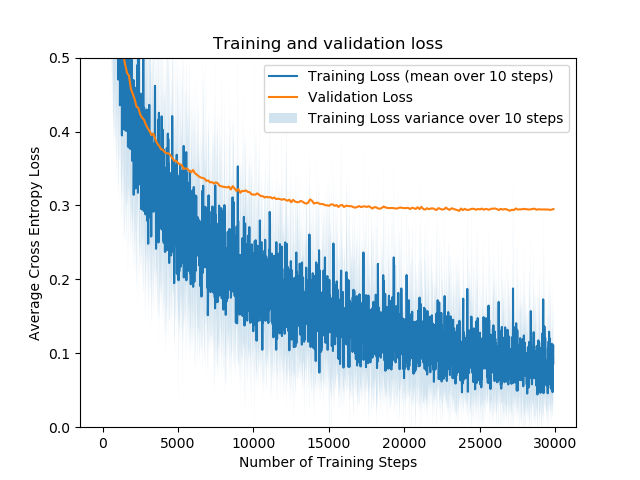
\includegraphics[width=\textwidth]{Assignments/Assignment_2/plots/task2abc/2c_loss.png}
    \caption{Training and validation loss of a neural network with two layers.}
    \label{fig:task2loss}
\end{figure}

\begin{figure}[H]
    \centering
    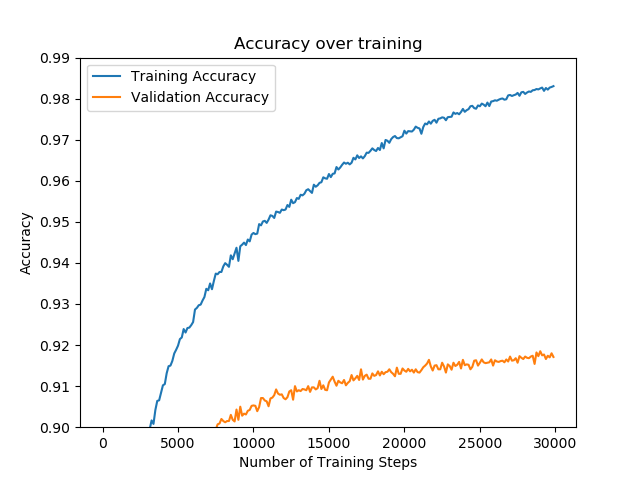
\includegraphics[width=\textwidth]{Assignments/Assignment_2/plots/task2abc/2c_accuracy.png}
    \caption{Training accuracy of a neural network with two layers.}
    \label{fig:task2acc}
\end{figure}

\subsection{Task 2d: Number of parameters}
The number of parameters in the network is defined as the number of weights plus the number of biases. In this case the network has two layers. 64 nodes in the hidden layer and 10 nodes in the output layer. The input vector $\boldsymbol{x}$ consists of 785 elements, 784 data points and 1 bias. The weights include biases, because the bias trick has been implemented. The resulting number of parameters $P$ is thus:
\begin{equation}
    P = 785\cdot64 + 64\cdot 10 = 50,880 
    \label{eq:num_params}
\end{equation}


\section{Adding the ”Tricks of the Trade”}

In order to improve the performance of the network a few "tricks" have been added to the model. To clearly document the effect of a given ``trick'', performance variations will be discussed with each addition. A complete overview of the final metrics in the network for each addition is outlined in \autoref{tab:3table}.

\subsection{Task 3a: Improved weight initialization}
The first addition to the model that will be discussed is improved initialization of the input weights. The initial weight matrix, $\text{\textbf{W}}_{t=0}$, is drawn from a normal distribution, $\text{\textbf{W}}_{t=0} \sim \mathcal{N}(\mu,\sigma)$, with mean $\mu = 0$ and standard deviation $\sigma = 1/\sqrt{\text{fan-in}}$. The number ``fan-in'' is the number of inputs to the given neuron, i.e for the hidden layer fan-in = 785 and for the output layer fan-in = 64.

The loss and accuracy on the training and validation data sets for the network with and without improved weight initialization is shown in \autoref{fig:3a_loss} and \autoref{fig:3a_acc}. 

From both plots it is clear that introducing the improved Sigmoid lowers both the final training loss and accuracy, aswell as the final validation loss and accuracy. Furthermore, by studying \autoref{fig:3a_loss} one can observe that the ``gap'' between the training and validation loss is larger without the improved weights, compared to the gap between the training and validation loss \textit{with} improved weights. \autoref{tab:3table} confirms this gap. This suggests that the model has been more generalized, and is consquently less overfitted after adding the improved weights. Finally one can also observe that the learning speed and convergence rate is improved since there is increased performance compared to the network without additions, with the same number of training steps.

\begin{figure}[H]
    \centering
    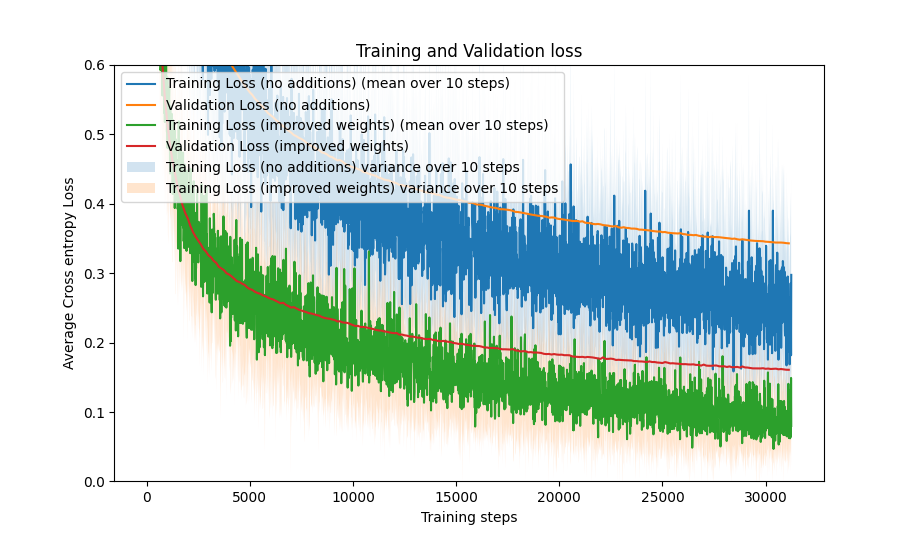
\includegraphics[width=\textwidth]{Assignments/Assignment_2/plots/task3/3a_loss.png}
    \caption{Training and validation loss with and without improved weight initialization.}
    \label{fig:3a_loss}
\end{figure}

\begin{figure}[H]
    \centering
    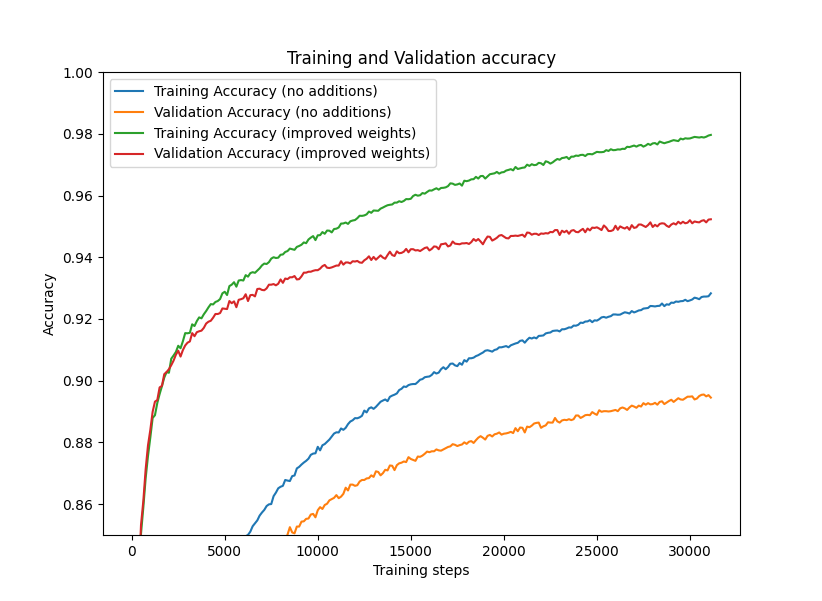
\includegraphics[width=\textwidth]{Assignments/Assignment_2/plots/task3/3a_accuracy.png}
    \caption{Training and validation accuracy with and without improved weight initialization.}
    \label{fig:3a_acc}
\end{figure}

\subsection{Task 3b: Improved Sigmoid}

The second addition to the model, is improving the Sigmoid activation function for the hidden layer. Previously, the Sigmoid function used was given by $f(x) = \frac{1}{1 + e^{-x}}$. The issue with such an activation function, is that its outputs are not centered around zero and alway positive. As discussed in \textit{LeCun 1998} [1], it is desirable to have outputs centered around zero, as this usually results in faster convergence. As a new activation function, the following hyperbolic function has been chosen: 
\begin{equation}
    f(x) = 1.7159 \tanh{(\frac{2}{3}x)}
    \label{eq:tanh}
\end{equation}


When performing the gradient descent, the derivative of the activation function is needed. Differentiating \eqref{eq:tanh} gives:
\begin{equation}
    f'(x) = 1.7159 \frac{2}{3 \cosh^2{(\frac{2}{3}x)}}
    \label{eq:tanh-der}
\end{equation}

The loss and accuracy on the training and validation data sets for the network with and without improved weight initialization and with and without improved weight intitialization and improved Sigmoid is shown in \autoref{fig:3b_loss} and \autoref{fig:3b_acc} respectively. 

From the plots it is clear that introducing the improved Sigmoid in addition to the improved weights lowers both the final training and validation loss, and increases the training and validation accuracy even further. However, by studying \autoref{fig:3b_loss} it is clear that the validation loss with both improved weights and improved Sigmoid remains unchanged for around 10 000 to 25 000 timesteps before early stopping kicks in. This results in a large gap between the validation loss and training loss, indicating that the model begins to overfit on the training data. Again there is an improvement in learning speed and convergence rate. One can observe that the model with improved Sigmoid and improved weights requires less training steps to achieve the same performance compared to only using improved weights.

\begin{figure}[H]
    \centering
    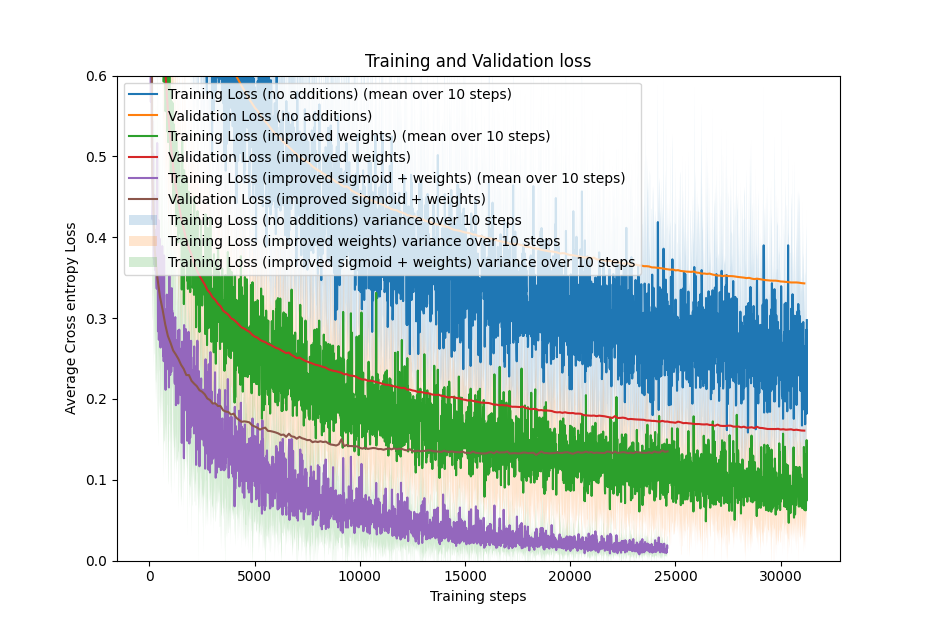
\includegraphics[width=\textwidth]{Assignments/Assignment_2/plots/task3/3b_loss.png}
    \caption{Training and validation loss with and without improved weight initialization and improved Sigmoid.}
    \label{fig:3b_loss}
\end{figure}

\begin{figure}[H]
    \centering
    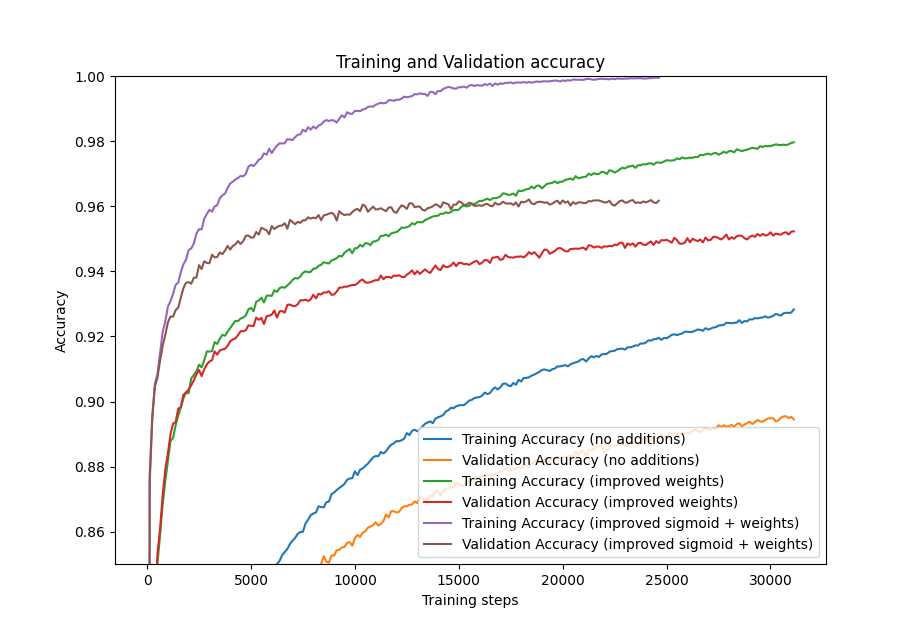
\includegraphics[width=\textwidth]{Assignments/Assignment_2/plots/task3/3b_accuracy.png}
    \caption{Training and validation accuracy with and without improved weight initialization and improved Sigmoid.}
    \label{fig:3b_acc}
\end{figure}


\subsection{Task 3c: Momentum}
The third and final addition to the model that will be discussed is momentum for the gradient descent. Momentum helps in utilizing a small portion of the previous gradients. This will make the gradient converge faster and may also prevent the network from getting stuck in a local minima as opposed to the desired global minima. The momentum is given by
\begin{equation}
    \Delta w (t + 1) =  \frac{\partial C}{\partial w} + \gamma \Delta w(t)
    \label{eq:momentum}
\end{equation}
 Furthermore, the update step for a given weight, $w_{ji}$, with momentum added becomes 

\begin{equation}
    \Delta w_{ji} :=  w_{ji} - \alpha \cdot \Delta w(t)
    \label{eq:momentum-grad}
\end{equation}


The resulting training and validation loss for the network with two additions (weights and Sigmoid) and all tree additions(weights, Sigmoid and momentum) are shown in \autoref{fig:3c_loss}. The resulting training and validation accuracy for the network with two additions (weights and sigmoid) and all tree additions(weights, Sigmoid and momentum) are shown in \autoref{fig:3c_acc}. To avoid overfilled plots, the network configuration without any additions and the network configuration with only improved weights have been omitted.

From \autoref{fig:3c_loss} it is clear that the loss for the training set converges towards zero and the validation loss is starting to increase after about 5000 training steps. This is a clear indication of overfitting. The validation loss is even higher than for the network without the added momentum. The cause of this can be that the training set is too small and/or the training set is not generalized enough. The number of epochs required to train the network is the lowest among the four networks. This proves that the addition of momentum works as intended.

\begin{figure}[H]
    \centering
    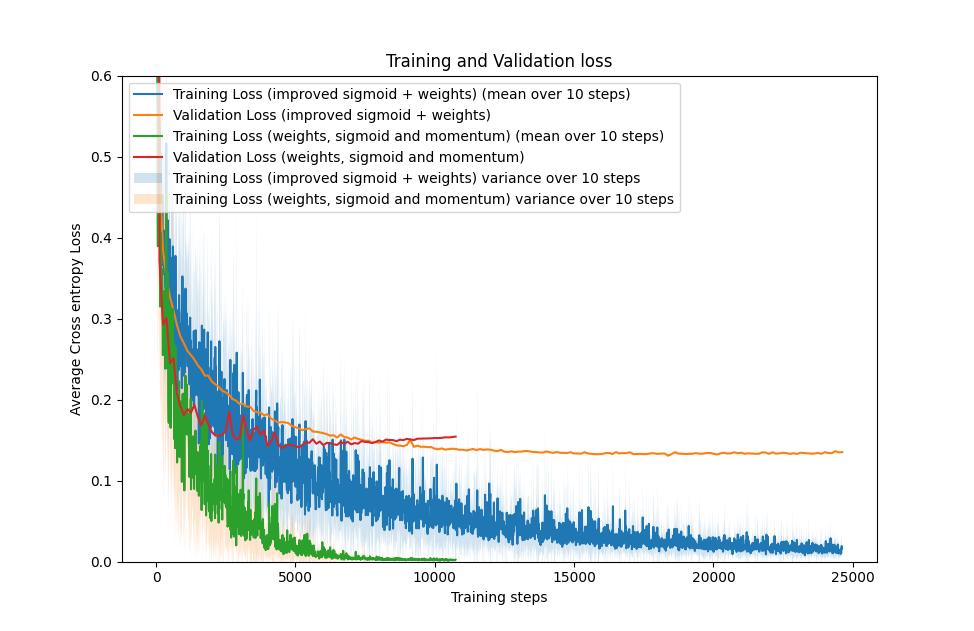
\includegraphics[width = \textwidth]{Assignments/Assignment_2/plots/task3/3c_loss.png}
    \caption{Training and validation loss with and without all three additions.}
    \label{fig:3c_loss}
\end{figure}

\begin{figure}[H]
    \centering
    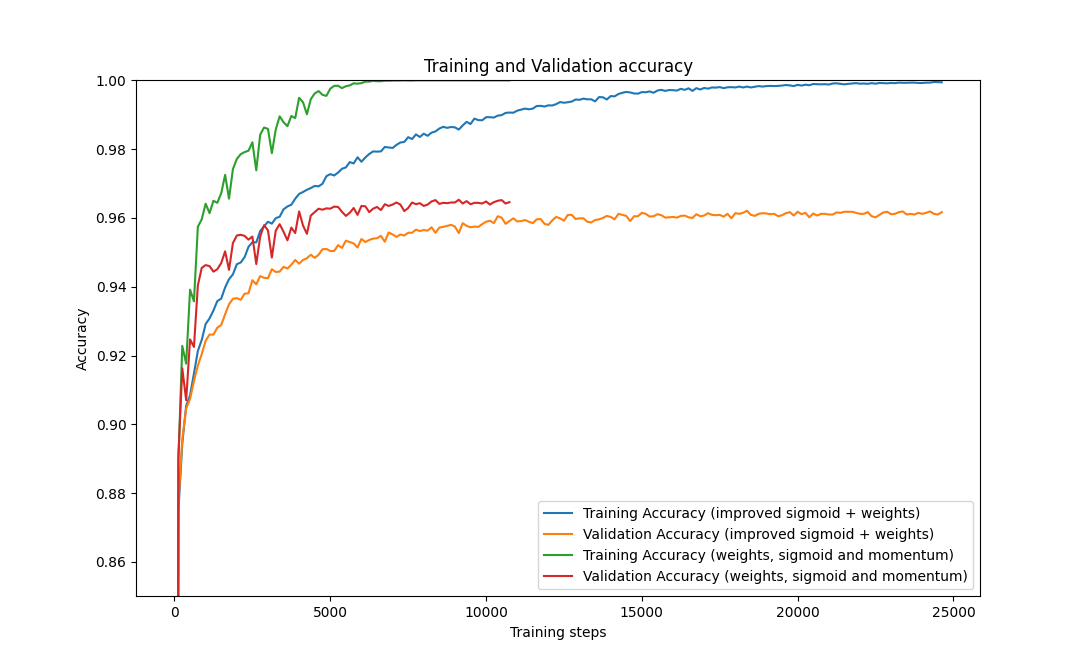
\includegraphics[width = \textwidth]{Assignments/Assignment_2/plots/task3/3c_accuracy.png}
    \caption{Training and validation accuracy with and without all three additions.}
    \label{fig:3c_acc}
\end{figure}









\begin{table}[H]
\caption{Network metrics for different network configurations}
\label{tab:3table}
\begin{tabular}{|l|l|l|l|l|l|}
\hline
\multicolumn{1}{|c|}{\textbf{Addition}} & \multicolumn{1}{c|}{\textbf{\begin{tabular}[c]{@{}c@{}}Validation \\ Loss\end{tabular}}} & \multicolumn{1}{c|}{\textbf{\begin{tabular}[c]{@{}c@{}}Validation \\ Accuarcy\end{tabular}}} & \multicolumn{1}{c|}{\textbf{\begin{tabular}[c]{@{}c@{}}Training\\ Loss\end{tabular}}} & \multicolumn{1}{c|}{\textbf{\begin{tabular}[c]{@{}c@{}}Training \\ Accuracy\end{tabular}}} & \multicolumn{1}{c|}{\textbf{Epochs}} \\ \hline
No additions & 0.3427 & 89.47\% & 0.2456 & 92.81\% & 50 of 50 \\ \hline
Improved weights & 0.1612 & 95.2\% & 0.0874 & 97.96\% & 50 of 50 \\ \hline
Improved Sigmoid & 0.1352 & 96.17\% & 0.0137 & 99.95\% & 39 of 50 \\ \hline
Momentum & 0.1544 & 96.46\% & 0.0018 & 100\% & 17 of 50\\ \hline
\end{tabular}
\end{table}


\section{Experiment with network topology}

\subsection{Task 4a \& 4b: Comparison of number of hidden nodes}

To compare a network with a low number of nodes in the hidden layer to a network with a high number of nodes in the hidden layer, a network with $J_{low} = 32$ nodes in the hidden layer has been compared to a network with $J_{high} = 128$. As a baseline for the comparison, $J_{baseline} = 64$ nodes in the hidden layer has been used, as this is the size of the hidden layer used previously in this assignment.

The loss and accuracy for the training and validation sets for different networks with a varying number of hidden nodes is shown in \autoref{fig:4ab-train} and \autoref{fig:4ab-val}. Final performance metrics are outlined in \autoref{tab:metrics4ab}.

From \autoref{fig:4ab-train}, \autoref{fig:4ab-val} and \autoref{tab:metrics4ab} it is evident that for a network with $J_{low} = 32$ units the performance, when compared to the baseline network of 64 hidden units. This is clear as neither the training loss nor the validation accuracy for the small hidden layer network reaches the levels of the baseline example. Additionally, the smaller network has a slower convergence speed (?). Thus it can be concluded that if the number of hidden units is too low, the network will perform poorly.

From \autoref{fig:4ab-train}, \autoref{fig:4ab-val} and \autoref{tab:metrics4ab} it is evident that for a network with $J_{high} =128$ units in the hidden layer, there is an increase in performance so small that it can be considered negligible. There is however, an increase in training time as the plots show that the graph of the 128-unit network requires an extra amount of timesteps compared to the baseline network. As evident in \autoref{tab:metrics4ab} the larger network uses an extra epoch before training terminates. Thus it can be concluded that if the number of hidden units is too large, the increase in performance is negligible while and the training time for the network increases. 


\begin{figure}[H]
    \centering
    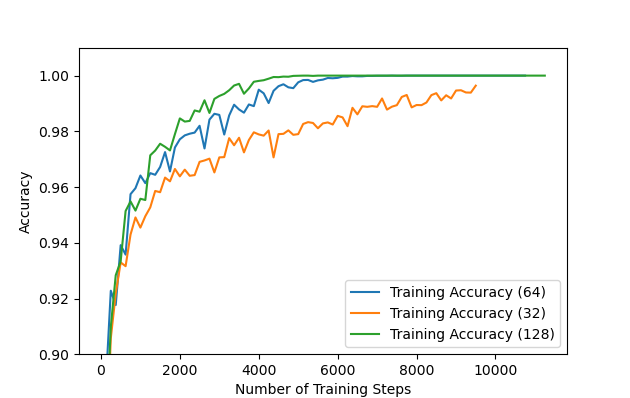
\includegraphics[width=\textwidth]{Assignments/Assignment_2/plots/task4/task4ab_train_acc.png}
    \caption{Comparison of performance impact on the training set accuracy with different number of hidden nodes.}
    \label{fig:4ab-train}
\end{figure}


\begin{figure}[H]
    \centering
    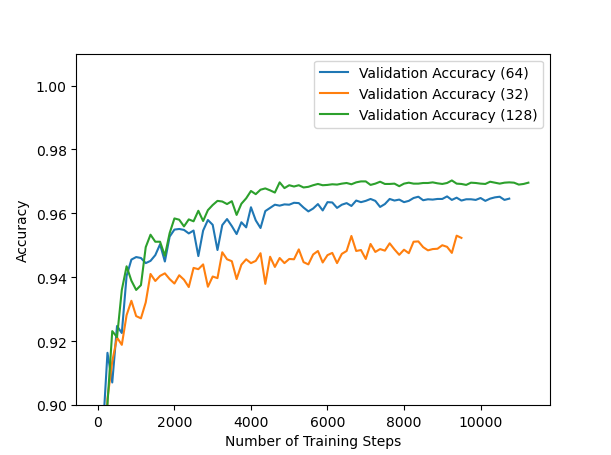
\includegraphics[width=\textwidth]{Assignments/Assignment_2/plots/task4/task4ab_val_acc.png}
    \caption{Comparison of performance impact on the validation set accuracy with different number of hidden nodes.}
    \label{fig:4ab-val}
\end{figure}


\begin{table}[H]
\caption{Final performance metrics for different number of hidden units.}
\label{tab:metrics4ab}

\begin{tabular}{|l|l|l|l|l|l|}
\hline
\multicolumn{1}{|c|}{\textbf{\# Hidden units}} & \multicolumn{1}{c|}{\textbf{\begin{tabular}[c]{@{}c@{}}Validation \\ Loss\end{tabular}}} & \multicolumn{1}{c|}{\textbf{\begin{tabular}[c]{@{}c@{}}Validation \\ Accuracy\end{tabular}}} & \multicolumn{1}{c|}{\textbf{\begin{tabular}[c]{@{}c@{}}Training\\ Loss\end{tabular}}} & \multicolumn{1}{c|}{\textbf{\begin{tabular}[c]{@{}c@{}}Training \\ Accuracy\end{tabular}}} & \multicolumn{1}{c|}{\textbf{Epochs}} \\ \hline
32                      & 0.1991       & 95.23\%                       & 0.0186   & 99.64\%                     & 15              \\ \hline
64                      & 0.1544      & 96.46\%                       & 0.0018   & 100\%                          & 17              \\ \hline
128                     & 0.1314      & 96.96\%                       & 0.0008  & 100\%                          & 18              \\ \hline
\end{tabular}

\label{tab:metrics4ab}
\end{table}



\subsection{Task 4d: Multi layer network}
A new network with two hidden layers have been implemented. It is desirable to have approximately the same number of parameters in the new network as the number of parameteres in the old, single-hidden-layer network, which from \eqref{eq:num_params} is 50,880. By letting each of the two hidden layers in the new network have a total of 59 units, the total number of parameters becomes

\begin{equation}
    P = 785 \cdot 59 + 59 \cdot 59 + 59 \cdot 10 = 50,386
\end{equation}
which is almost the same number of parameters as in the old network.


A comparison between the two networks is shown in \autoref{fig:4d_lossy} and \autoref{fig:4d_acc}. Additionally, the final performance metrics are outlined in \autoref{tab:metrics4d}.


From \autoref{fig:4d_lossy}, \autoref{fig:4d_acc} and \autoref{tab:metrics4d} it is clear that the difference in the final accuracy of the networks is negligible. However, there is a difference in the final loss. The loss for the double hidden layered network is higher than the single hidden layered network. This could indicate, that while they both predict the same number of digits correctly, the single layer network is more ``confident'' in its predictions.

\begin{figure}[H]
    \centering
    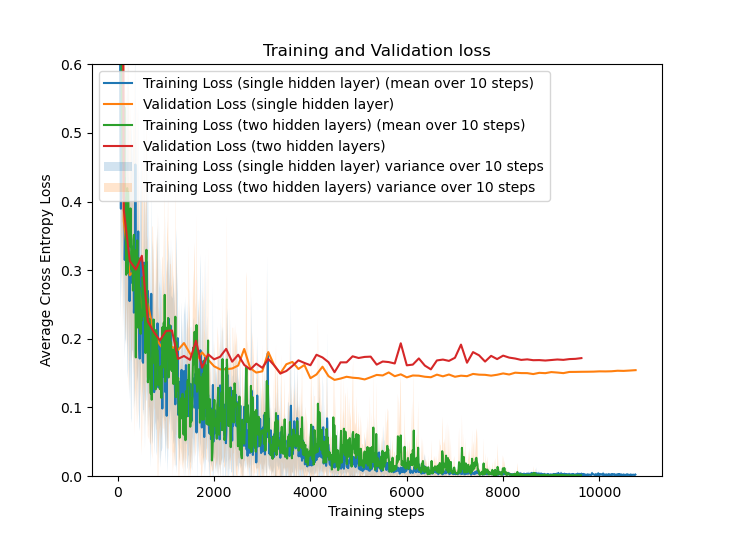
\includegraphics[width=\textwidth]{Assignments/Assignment_2/plots/task4/task4d_loss.png}
    \caption{Validation and training loss for networks with approximately the same number of parameters but different topology.}
    \label{fig:4d_lossy}
\end{figure}


\begin{figure}[H]
    \centering
    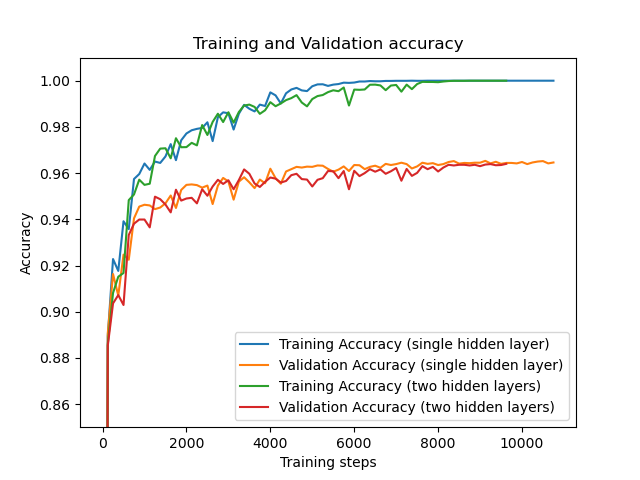
\includegraphics[width=\textwidth]{Assignments/Assignment_2/plots/task4/task4d_acc.png}
    \caption{Validation and training accuracy for networks with approximately the same number of parameters but different topology.}
    \label{fig:4d_acc}
\end{figure}
 
 
 
 \begin{table}[H]
 \caption{Final performance metrics for single hidden layer network and double hidden layer network. Both networks have the same number of parameters.}
\label{tab:metrics4d}
\begin{tabular}{|l|l|l|l|l|l|}
\hline
\multicolumn{1}{|c|}{\textbf{\# Hidden units}} & \multicolumn{1}{c|}{\textbf{\begin{tabular}[c]{@{}c@{}}Validation \\ Loss\end{tabular}}} & \multicolumn{1}{c|}{\textbf{\begin{tabular}[c]{@{}c@{}}Validation \\ Accuracy\end{tabular}}} & \multicolumn{1}{c|}{\textbf{\begin{tabular}[c]{@{}c@{}}Training\\ Loss\end{tabular}}} & \multicolumn{1}{c|}{\textbf{\begin{tabular}[c]{@{}c@{}}Training \\ Accuracy\end{tabular}}} & \multicolumn{1}{c|}{\textbf{Epochs}} \\ \hline
64    & 0.1543    & 96.46\%         & 0.0009      & 100\%          & 17         \\ \hline
59, 59  & 0.1719      & 96.40\%    & 0.0018     & 100\%    & 15        \\ \hline
\end{tabular}

\end{table}


\subsection{Task 4e: 10 layer network}
A network with 10 hidden layers with 64 hidden units for each layer has been implemented. A comparsion of performance between the 10 layer network and the baseline one layer network from task 3 is shown in \autoref{fig:tenlayers_acc} and \autoref{fig:tenlayers_loss}. Additionally, in \autoref{tab:4emetrics} the final performance metrics for the model is shown.  

The results show that the 10 layer network uses significantly more training steps before the training ends. This is a consequence of the large number of parameters in the model. Even though there are more parameters, the network has worse performance, both in terms of loss and accuracy. The model is likely too complex for the given problem, and the dataset maybe too small and not generalized enough. From \autoref{tab:4emetrics} one can see that in the 10 layer model, there are a total of 87,744 parameters. This is a 72\% increase from the baseline model, supporting the claim that the model is too complex. The fact that the number of epochs for training is up with 88\%, but with no improvement of results, indicates that the number of weights is simply too great. 


\begin{figure}[H]
    \centering
    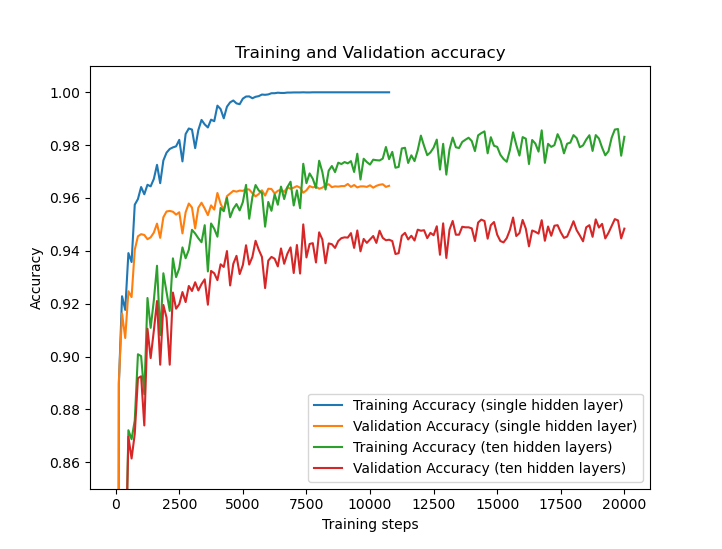
\includegraphics[width=\textwidth]{Assignments/Assignment_2/plots/task4/task4e_acc.png}
    \caption{Training and validation accuracy for a single hidden layer network and a 10 hidden layer network.}
    \label{fig:tenlayers_acc}
\end{figure}


\begin{figure}[H]
    \centering
    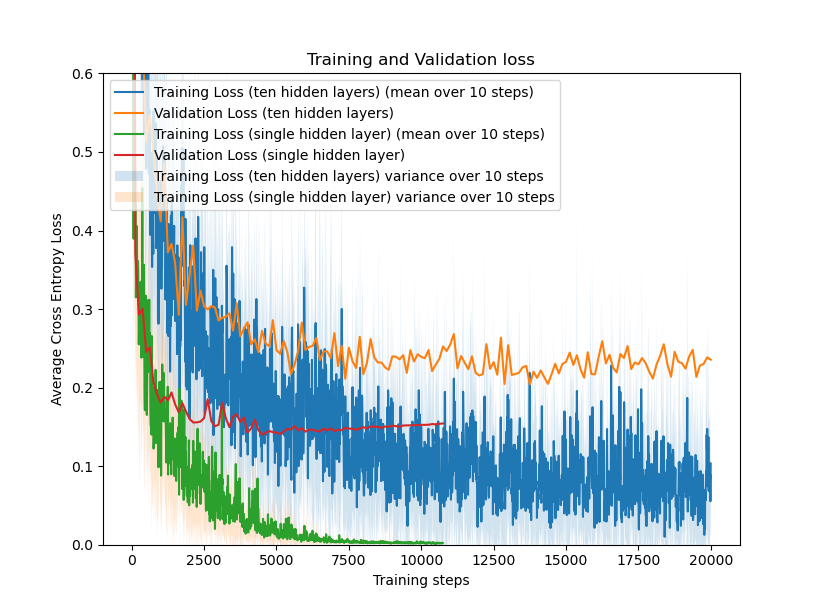
\includegraphics[width=\textwidth]{Assignments/Assignment_2/plots/task4/task4e_lossy.png}
    \caption{Training and validation loss for a single hidden layer network and a 10 hidden layer network.}
    \label{fig:tenlayers_loss}
\end{figure}


\begin{table}[H]
\caption{Final performance metrics for the 10 hidden layer neural network and a single layer neural network.}
\label{tab:4emetrics}
\begin{tabular}{|l|l|l|l|l|l|}
\hline
\multicolumn{1}{|c|}{\textbf{\# Hidden units}} & \multicolumn{1}{c|}{\textbf{\begin{tabular}[c]{@{}c@{}}Validation \\ Loss\end{tabular}}} & \multicolumn{1}{c|}{\textbf{\begin{tabular}[c]{@{}c@{}}Validation \\ Accuracy\end{tabular}}} & \multicolumn{1}{c|}{\textbf{\begin{tabular}[c]{@{}c@{}}Training\\ Loss\end{tabular}}} & \multicolumn{1}{c|}{\textbf{\begin{tabular}[c]{@{}c@{}}Training \\ Accuracy\end{tabular}}} & \multicolumn{1}{c|}{\textbf{Epochs}} \\ \hline
64 & 0.1543 & 96.46\% & 0.0018 & 100\% & 17 \\ \hline
64 \cdot 10 & 0.2355 & 94.84\% & 0.0591 & 98.32\% & 32 \\ \hline
\end{tabular}
\end{table}



\begin{thebibliography}{9}
\bibitem{sauce}
[LeCun et al., 2012] LeCun, Y. A., Bottou, L., Orr, G. B., and Müller, K.-R. (2012). Efficient backprop.
\textit{In Neural networks: Tricks of the trade}, pages 9–48. Springer.
\end{thebibliography}
\end{document}